\section{Design Consideration and Options}
\label{sect:options}

As discussed earlier, collocating the backup service on the existing
cloud cluster avoids the extra cost to acquire a dedicated backup facility
and reduces the network bandwidth consumption in transferring the un-deduplicated
raw data for backup. 
Figure~\ref{fig:collocated} illustrates the cluster architecture where
each physical runs a backup service and a distributed file system (DFS)~\cite{GFS2004,Hadoop} 
serves a backup store  for the snapshots.
The previous study shows that 
 deduplication can compress the backup copies 
effectively in a 10:1 or even 15:1 rage. 
Therefore  the portion of space in a cluster
allocated for snapshots of data should not dominate
the cluster storage usage.


%The running of such a service is subject to the resource availability of the system and 

% That arises mainly in Alibaba's Aliyun cloud service.
%concerns
%Base on Aliyun's production environment, the snapshot backup job has to satisfy 


\begin{figure}[htb]
    \centering
    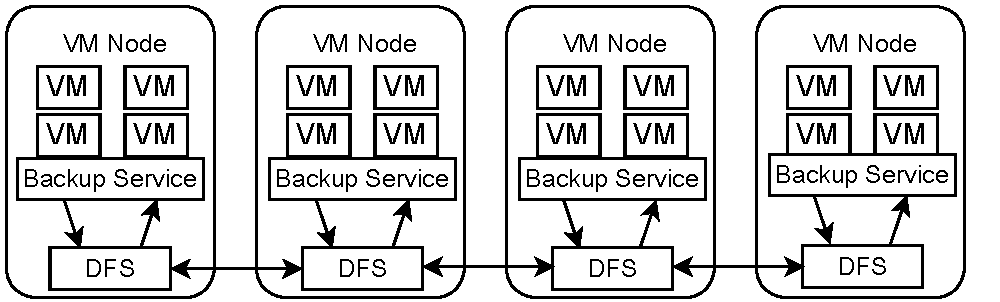
\includegraphics[width=3in]{images/colocated-arch}
    \caption{Collocated VM Backup System.}
    \label{fig:collocated}
\end{figure}

%{\em Collocating with cluster-based cloud services.}
%We collocate the backup service with other cloud services in a cluster
%and use a distributed file system
%store the backup with multiple replicas. 
%There might be a concern that storing many versions of snapshots would
%go against the purpose of deduplication.

%Assume on the average the compression
%ratio is $c$:1.  When the number of versions
%saved in the backup storage is $l$  on the average, 
%the amount of storage space in the cluster allocated  for the backup would be $\frac{l}{l+c}$.
%For example, when $l=5$ and $c=10$, 33\% of the cluster storage is used for the backup.
%When $l=9$ and $c=13$, storage usage is 40\%. 
%That is acceptable given today's cheap cost for disk storage.
%In the case of Alibaba, each machine hosts 25 VMs on the average and each VM uses 40GB data.
%Each machine however can typically provide over 10TB storage.
%Thus the normal disk usage  is about 1TB per machine, and adding 30\% to 100\% 
%extra space for the backup is not a practical concern, especially with the
%added benefits of cheaper running costs and lower network bandwidth requirements.

We discuss the design considerations as follows. 
\begin{itemize}
\item {\em Deduplication localization, sharing minimization, and fault tolerance.}

%Previous work in deduplication~\cite{extreme_binning09,sparseindex09} has
%studied the solutions to reduce memory requirements.
%One important issue not considered in the previous work is how 
Because a data chunk is compared with signatures collected from other VMs during
the deduplication process, only one copy of duplicates is stored in the backup storage
and this artificially creates data dependency among different VM users. 
Content sharing via deduplication affects fault isolation since machine failures happen at daily 
basis in a large-scale cloud and
%failure of a shared block affects many VMs.
%the loss of a shared chunks can affect many VM users whose snapshots share this 
%data block. 
loss of a small number of shared data chunks can 
cause the unavailability of snapshots for a large number of virtual machines.
Localizing the impact of deduplication can increase fault isolation and resilience.
Thus from the fault tolerance point of view,  duplicate sharing among multiple VMs is 
discourage. 
Another disadvantage of sharing is that it complicates snapshot deletion.
The mark-sweep approach~\cite{mark-sweep} is effective for deletion, and its main cost
is to count if a data chunk is still shared by other snapshots.
Thus our goal is to localize deduplication and minimize sharing, while we seek for 
a tradeoff since there are a significant number of duplicates cross VMs.
 
% since storage for shared identical content chunks can become a failure point.
%Without any control of such data sharing, we can only increase  
%replication for global datasets to enhance the availability,
%but this incurs significantly higher costs.
%Thus a key goal  in our design
%is restricting the impact of  data loss to a limited number of VMs. 
%It is not desirable that small scale of data failure affects the backup of many VMs.
%when users access snapshots in a recovery process. 
\item{\bf Packaging  data chunks as file system blocks.}
Since the file block size in the Hadoop and GFS is uniform and large with 64MB as a default setting,
the content chunk in a deduplication system is of nonuniform size with 4KB or 8KB on average.
We need to build an intermediate layer that supports large snapshot writing with append operations
and infrequent snapshot access.
Packaging that maps data chunks to file system blocks can create data dependence among VMs
since a file block can be shared even more VMs.
Thus we need to consider a minimum association of a fie system block to VMs in the packaging process.
%The distributed file system~\cite{GoogleFS,Hadoop} provides the replication support
%and we can leverage existing open-source software to implement such a layer.
%When the number of machines failed exceeds the replication degree, there could be
% some data loss.  
%Storage deduplication worsens the impact of such faults
%because  the majority of each snapshot (e.g. over 90\%) is deduplicated
%and the corresponding data chunks stored in the underlying file blocks
%are shared by many VMs. 
%The failure of one data chunk or block can impact many sharing VMs. 
\end{itemize}

%\item {\em Requirement for backup throughput and low computing resource usage}.
Because of collocation of this snapshot service with other existing cloud services, 
%As a large-scale cluster hosting tens of thousand of active VMs everyday,  the amount of data
%to be processed can be huge. 
cloud providers wish that the backup service only consumes  small resources
with a minimal impact to the existing cloud services.
%the computing resources allocated for the snapshot service is limited, especially
%because of its lower priority.
The key usage of resource for backup is memory for storing and comparing the fingerprints. 
We will consider the approximation techniques with less memory consumption
studied in~\cite{extreme_binning09,Guo2011} along with the fault isolation consideration discussed below. 
%A snapshot backup service shall not compete cpu, memory, or I/O bandwidth with VMs. 
%Fingerprint-based search does require a significant amount of memory for fingerprint lookup
%and comparison.  This competes memory resource  with the existing VMs.
%Our design is to identify a low-cost and low-profile scheme for deduplication.
%Specifically, the memory usage of snapshot service can never exceed 500MB in any node.
%Excessive use of bandwidth and computing resource for backup can create
%noticeable contention for resources with the existing cloud, which is not
%preferred and may not not be acceptable for production system operation. 
%Thus it is desirable that backup for all nodes
%can be conducted in parallel and in a short period of time,
%and any centralized or cross-machine communication for
%deduplication should not become a bottleneck.
%For example, in an Aliyun cluster with over 1,000 nodes and each hosts over 25 VMs, 
%the system must finish saving daily snapshots of all VMs in a few hours. 
%Often a cloud has a few hours of light workload each day (e.g. midnight),  
%which creates an small window for automatic backup.
%The backup service can generate hundreds of terabytes of data in such a time window
%without optimization and thus the resource content is considered carefully as we design
%a fault-resilient cluster-based solution. 
%In our typical 1000 nodes cluster, each node hosts 25 VMs, each VM has 40GB of data on average, that translates to backup throughput of 139GB/second, or 
%500TB/hour.  The system must finish saving daily snapshots of all VMs in few hours. 

%At Aliyun, it is required that while CPU and disk usage should be small or modest during backup time,
%the memory footprint of snapshot service should not exceed 500MB at each node.


\comments{
Another consideration is backup data cleaning to delete useless blocks.
Keeping reference counters for shared data blocks is challenging and less reliable.
The previous work has advocated the mark-and-sweep approach  which periodically
scans all data (or modified latest version of data)~\cite{?, Guo2011}. It first marks
all used blocks and then sweep all chunks to reclaim unmarked blocks. 
This approach is resilient to errors: at any time the process can simply be restarted with no 
negative side effects.  Scalability, however, is an issue.
To deal with 1 PB snapshots data, which may be represented by 10,000 GB FP index,
If we account for an average deduplication factor of 10 (i.e., each chunk
is referenced by 10 different snapshots), the total size
of snapshot metadata that need to be read during the mark phase will
be 100 TB.  This alone will take almost 2 hours on a
1000-machine cloud. Furthermore, marking the in-use
bits for 250 billion entries is no easy task. There is no
way to put the bit map in memory. One might want
to mitigate the poor performance of mark-and-sweep by
doing it less frequently. But in practice this is not a viable
option: customers always want to keep the utilization
of the system close to its capacity so that a longer
history can be stored. With daily snapshots taking place,
systems rarely have the luxury to postpone deletion operations
for a long time. In our field deployment, deletion
is done once a day. More than 2 hours in each run is too
much. In a large production-oriented deduplication system reference
management needs to be very reliable and have
good recover-ability. It should tolerate errors and always
ensure correctness. Although mark-and-sweep provides
these properties, its performance is proportional to the
capacity of the system, thus limiting its scalability.

}



%we want to isolate 
%each VM's snapshot backup as much as possible while still enjoy the benefit of deduplication.
%In large scale cloud, node faiures happen at daily basis, we don't want a problem at small scale
%to affect large amount of VMs due to data sharing.
%a key weakness of global content fingerprint comparison is that it affects fault isolation.

%2) data sharing among users for accessing common signagutes causes the system less resilient to storage failures.
%any loss of one piece of  shared data content hash and actualcontent will damange many VM snapshots, which can cause massive impacts
%on reliability of many users.

%Another point is that the previous work in signature-based comparison does not address
%load balancing for a distributed environment during parallel access.  
%Some content signatures can be extremely hot, but the machines  that  handle such signatures can become
% a bottleneck. Uncoordinated signature assignment could lead to imbalanced access workload.


%There are multiple choices of snapshot backup design for VM images and our considerations are described
%as follows. 
%Our design considerations
%\begin{enumerate}
%\item {\bf Centralized vs. decenalized} 
%
%It is desirable to have  a decentralized architecture.
%Given a large amount of snapshot data communicated from each machine to the backup storage,
%with a distributed storage architecture for backup, one could exploit  exploit data locality between
%the source of data and storage location of data to reduce cross-platform bandwidth requirement for backup.

%execute in parallel and easy to coordinate. In fact, we want to avoid cross-node dependency at scheduling VM snapshot operations, such that no global coordinator is necessary.
%\item {Load balancing in resource consumption}: the cost of snapshot service shall be evenly distributed onto every node. We don't have a super powerful
%or stable node that can accept extra responsibility.
%\item {minimization of inter-user data dependency for fault tolerance}: we want to minimize the data dependency to a controllable level. Data deduplication means sharing of data, thus one failure at a single point may affect the snapshot service of hundreds of VMs, which is absolutely unacceptable.
%\item {Resource usage modeling and control}.
%\end{enumerate}


A deduplication scheme compares the fingerprints of the current snapshot
with its parent snapshot and also other snapshots in the entire cloud without consideration of .
%The traditional approach compares all fingerprints and
%stores one copy for all of a chunk's duplicates.
We call this as  the VM-oblivious (VO) approach.
In designing and selecting a duplication algorithm, we have considered the following options.
\begin{itemize}
\item {\bf Version-based change detection}.
VM snapshots can be  backed up  incrementally by identifying file  blocks that have
changed from the previous version of the snapshot~\cite{Clements2009,Vrable2009,TanIPDPS2011}.
Active snapshots will contain all the information needed to restore the virtual disk
and when deleting a snapshot, data referenced by other snapshots are removed.
While full signature comparison can deliver additional reduction~\cite{Guo2011,Dong,ExtremeBining},
content change detection falls into a VM-centric approach since deduplication is localizable. 
We are seeking for additional optimization to improve duplication efficiency and design the 
association of data chunks with the underlying file blocks so that
file block sharing among VMs is minimized.
\item {\bf sampled Index}.
One alternative approach to reducing the use of memory space is 
to use a sampled index with prefetching, proposed  by Guo and Efstathopoulos\cite{Guo2011}. 
An evaluation with our test data shows that using a sampled index can achieve a high
deduplication efficiency with a single machine setup.  
One key problem is that the algorithm is VM oblivious and not easy to be adopted for VM-centric.
Another problem is  to design a distributed version 
in deduplicating large bodies of data. 
%The algorithm stores the sampled index in memory, which is required for high
%throughput to avoid the disk-bottleneck problem - since the index itself has no
%locality information, lookups are essentially random, so the index must be
%somehow optimized to prevent excessive disk seeking (the sampling algorithm does
%this by storing the index in memory). 
To use a distributed memory version of the sampled index, every deduplicate request
may access a remote machine for index lookup,  which  incurs a significant overhead.


Another possibility is to use this approach partially  in our VM centric solution by indexing
the most popular data chunks. For a small set of popular data chunks, the prefetching strategy
used in the sampled index will not work well because the spatial locality is limited among popular 
data chunks. In our test data,  on average the number of consecutive data chunks is 7, which is too small
to be effective for index sampling. 

%To distribute this sampled index, every  each machine would
%either require a complete copy of the index which would have a prohibitive cost in
%memory, or something like memcached must be used, which leaves the same problem
%as the disk bottleneck with every index check potentially using the network.
%The difficulty in storing extremely large bodies of data
%is related, as once 1PB is stored in the system, assuming a sampling rate of 
%1/101 with 22 byte index entires, 55GB of (in memory) index are required.

%Our solution uses more total memory (??how much??), but is more scalable both in
%terms of capactity and distributing the deduplication. The only part of our
%algorithm which requires significant network traffic is the CDS deduplication,
%but this is done after Levels 1 and 2 (dirty bits and comparison to parent), and
%so is only done for a small percent of blocks (?? 5-10\% ??).

\item {\bf Stateless  Data Routing}.
Another approach for duplicate comparison  is to use a content-based hash
partitioning algorithm called stateless data routing~\cite{Dong20??}
that divides the deduplication work with an approximation, which 
is similar to Exreme Binning\cite{extreme_binning09}. 
Again such an approach is VM-oblivious while each request does incur a network routing latency, and then
additional overhead for a bloomer filter based  disk lookup~\cite{Dong20??} or 
a disk index access~\cite{extreme_binning09}. 
 
%We compared our solution to
%content-based hash partitioning by running the algorithm on our set of 
%traces. We used 2MB superchunks and 4KB chunks to partition the data, and use
%the minhashes of the superchunks for routing. The results of this are shown in
%Table~\ref{??}. Routing each chunk to a bin provides good deduplication
%efficiency, and only requires each storage node to keep an index of local data
%and the bin mapping, but misses significant opportunities in our indended use
%case.

%The problem with the Data Routing algorithm is in the very high network traffic.
%Our intended use case is a backup system which runs alongside a number of VMs,
%in order to save costs. Data Routing makes no use of the inherent locality in
%such a system, and therefore puts a much higher network burden on machines which
%are also running 35 VMs each. This will reduce the available network bandwidth
%to users of the VMs, and/or reduce the possible deduplication throughput.
\end{itemize}

With these considerations in mind, we study a 
VM-centric approach (called VC)
for a backup service co-hosted   in the existing set of machines and resource usage is friendly
to the existing applications.  
We will first discuss and analyze the integration of the VM-centric deduplication strategies with fault isolation, and then present
an architecture and implementation design with deletion support.

%The deduplication process is first conducted among snapshots within each VM
%and then is conducted across VMs.  
%Given the concern that searching duplicates across VMs is a global feature which can affect parallel performance
%and complicate failure management,
%we only eliminate the duplication of a small but popular data set while still maintaining a cost-effective deduplication ratio.
%For this purpose, we exploit the data characteristics of snapshots and collect most popular data.
%Data sharing across VMs is limited within this small data set such that adding replicas for it could enhance fault tolerance.
%
%in the  our studies show that there are a large amount of data unmodified in VM snapshots
%and shared among many users (e.g. OS data). The sharing pattern follows a zip-like distribution.
%With this characteristic, we can store a small amount of popular data items which coverage a large amount of
%snapshot data blocks. 
%We discuss our design and data analysis in the next section.


%This method is based on the observation of two facts in Aliyun's VM cloud: first, VM's OS disks contain 
%huge amount of operating system and software related data which is almost never modified during VM's life span. 
%Second, the duplication pattern of user generated data follows Zipf-like law, thus a tiny set of hottest data
%take up the majority of data duplication. As a result, if we extract these hot data as a common data set,
%then most of data duplication will emerge by searching in this very small scope.


%For example, In cloud storage, we are solving data deduplication problem in a different context of 
%data stream deduplication (the D2D case): our snapshot storage service is co-located with runtime VMs,
%thus we have very limited amount of system resource leave for data deduplication. For example,
%in Aliyun's 8-core, 48GB memory, 12TB VM server, there lives over 20 VMs who are hungrily competing for
%system resources: some may running map-reduce jobs, some may serving busy web requests, 
%some may storing backend databases, any behavior that affects user VMs performance or stability is unacceptable.

%To reduce the cost of deduplication, we must confine the scope of searching duplicates as much as possible,
%thus some hints are needed to tell us where the most likely duplicates would hide. 
%Several form of hints have been used in the past: many D2D systems exploits locality,
%which bases on the fact that duplicates are likely to appear in the same sequence as they have arrived before.
%Similarity is another popular hint, it suggests that two sets of data blocks may contain lots of
%duplicates if they are indetified as similar by certain similarity detection measurements.



%\section{Architecture design and Deduplication for Snapshot Support}
%
%\section{Popularity analysis}
% data on what data popular.
%
%Analysis: modeling: singular
%
%Compute: Cache hit ratio vs. cache cost (memory cost).


\comments{
\section{Challenges}
\subsection{Indexing}
Most deduplication systems operate at the sub-file level:
a file or a data stream is divided into a sequence of fixed
or variable sized segments. For each segment, a cryptographic
hash (MD5, SHA-1/2, etc.) is calculated as its
fingerprint (FP), and it is used to uniquely identify that
particular segment. A fingerprint index is used as a catalog
of fingerprints stored in the system, allowing the detection
of duplicates: during backup, if a tuple of the form <
FP, location > exists in the index for a particular
FP, then a reference to the existing copy of the chunk
is created. Otherwise, the chunk is considered new, a
copy is stored on the server and the index is updated accordingly.
In many systems, the FP index is also crucial
for the restore process, as index entries are used to locate
the exact storage location of the chunks the backup
consists of.

The index needs to have three important properties:
1) scale to high capacities, 2) achieve good indexing
throughput, and 3) provide high duplicate detection
rate—i.e., high deduplication efficiency. Table 1 demonstrates
how these goals become very challenging for a
Petascale system. Consider a typical virtualized cloud 
in which 10,000 VMs store 1 PB data, and the
chunk size is 4 KB (for fine-granularity duplicate detection),
indexing capacity will need to be at least 10,000
GB to support all 250 billion objects in the system. Such
an index is impossible to maintain in memory. Storing it
on disk, however, would greatly reduce query throughput.
To support 1000 concurrent snapshot backup tasks, 
an aggregate throughput of 20 GB/sec, would require the
index and the whole deduplication system for that matter
to provide a query service throughput of at least 5,000
Kops/sec. Trying to scale to 1 PB by storing the index
on disk would make it impossible to achieve this level
of performance. Making the chunk size larger (e.g.,
128 KB) would make deduplication far more coarse and
severely reduce its efficiency.

Even we can distribute the index over the cloud machines,
the resources that can be allocated to system services are
limited to minimize the negative impact to user experiences. 
So it becomes obvious that efficient, scalable indexing is
a hard problem. On top of all other indexing challenges,
one must point out that chunk FPs are cryptographic
hashes, randomly distributed in the index. Adjacent index
entries share no locality and any kind of simple readahead
scheme could not amortize the cost of storing index
entries on disk.


\subsection{Deletion}
Contrary to a traditional backup system, a dedupe system
shares data among files by default. 
Since snapshots in VM cloud face constant deletion, 
reference management
is necessary to keep track of chunk usage and reclaim
freed space. In addition to scalability and speed, reliability
is another challenge for reference management.
If a chunk gets freed while it is still referenced by snapshots,
data loss occurs and files cannot be restored. On the other
hand, if a chunk is referenced when it is actually no
longer in use, it causes storage leakage.

For simplicity, many previous works only investigated simple reference
counting without considering reliability
and recoverability. Reference counting, however, suffers
from low reliability, since it is vulnerable to lost or repeated
updates: when errors occur some chunks may
be updated and some may not. Complicated transaction
rollback logic is required to make reference counts consistent.
Moreover, if a chunk becomes corrupted, it is
important to know which files are using it so as to recover
the lost segment by backing up the file again. Unfortunately,
reference counting cannot provide such information.
Finally, there is almost no way to verify if the
reference count is correct or not in a large dynamic system.
Our field feedback indicates that power outages and
data corruption are really not that rare. In real deployments,
where data integrity and recoverability directly
affect product reputation, simple reference counting is
unsatisfactory.

Maintaining a reference list is a better solution: it is
immune to repeated updates and it can identify the files
that use a particular segment. However, some kind of logging
is still necessary to ensure correctness in the case of
lost operations. More importantly, variable length reference
lists need to be stored on disk for each chunk.
Every time a reference list is updated, the whole list (and
possibly its adjacent reference lists—due to the lists’
variable length) must be rewritten. This greatly hurts the
speed of reference management.

Mark-and-sweep is generally a better solution. 
During the mark phase, all snapshot metadata are traversed 
so as to mark the used chunks. 
In the sweep phase all chunks are swept and unmarked chunks are reclaimed. 
This approach is very resilient to errors: 
at any time the process can simply be restarted with no negative side effects. 
Scalability, however, is an issue.
To deal with 1 PB snapshots data, which may be represented by 10,000 GB FP index,
If we account
for an average deduplication factor of 10 (i.e., each chunk
is referenced by 10 different snapshots),
the total size
of snapshot metadata that need to be read during the mark phase will
be 100 TB. 
This alone will take almost 2 hours on a
1000-machine cloud. Furthermore, marking the in-use
bits for 250 billion entries is no easy task. There is no
way to put the bit map in memory. One might want
to mitigate the poor performance of mark-and-sweep by
doing it less frequently. But in practice this is not a viable
option: customers always want to keep the utilization
of the system close to its capacity so that a longer
history can be stored. With daily snapshots taking place,
systems rarely have the luxury to postpone deletion operations
for a long time. In our field deployment, deletion
is done once a day. More than 2 hours in each run is too
much. In a large production-oriented dedupe system reference
management needs to be very reliable and have
good recoverability. It should tolerate errors and always
ensure correctness. Although mark-and-sweep provides
these properties, its performance is proportional to the
capacity of the system, thus limiting its scalability.

\subsection{Fault Tolerance}
Because deduplication storage system
 artificially creates data dependency among different VM users,
it increases the risk of data availability.
In large scale cloud, node failures happen at daily basis,
the loss of access to a shared chunk can affect many VMs whose snapshots share this chunk. 
Without any control of the scope of data sharing, we can only increase the level of 
replication to enhance availability, which would significantly 
balance out the benefits of deduplication.

}
